\chapter{Testy}

Sprawdzenie poprawności działania obu algorytmów miało przebieg dwustopniowy:
\begin{itemize}
	\item symulacja modelu behawioralnego,
	\item uruchomienie algorytmu z warstwą sterującą na dronie.
\end{itemize}

\section{Testy symulacyjne}
O ile drugi ze sposobów był traktowany jako etap finalny, zwieńczający pracę nad projektem, to testy symulacyjne przebiegały równolegle z postępem prac nad poszczególnym z algorytmów śledzących. Co więcej, za wzór symulacji obrano uprzednio stworzony model programowy w MATLABie, chociażby ze względu na wykorzystanie tych samych obrazów w celu porównania wyników.
Moduł symulacyjny stworzony w środowisku Vivado i języku SystemVerilog nie uwzględniał jedynie części logiki zawartej w Block Designie - a więc instancji procesora oraz wejściowego i wyjściowego fragmentu toru wizyjnego. Byłaby to jednak część niepotrzebna, znacznie obciążająca i spowalniająca pracę symulatora. Jako zamiennik, wystarczył zasymulowany komplet sygnałów RGB z informacją o wartości piksela, która została wczytana z pliku tekstowego. Plik przechowujący jedną ramkę obrazu, wygenerowano w MATLABie umieszczając każdy kolejny pixel w nowej linii w formacie heksadecymalnym, po dwa znaki na każdą składową R, G i B.

Podstawowej funkcją symulacji jest możliwość podejrzenia propagowanych w układzie sygnałów w przystosowanym do tego oknie. Jednak ze względu na rozrastający się poziom skomplikowania modułów z czasem postanowiono bezpośrednio porównać wybrane funkcjonalności z pracą modelu programowego. W kodzie architektury stworzono logikę zapisującą do plików określone informacje z pojedynczej iteracji algorytmu. By jednak zapis nie był realizowany na każdym zboczu narastającym zegara, potrzebne było określenie sygnałów wyzwalających - zazwyczaj były to odpowiedniki sygnałów aktywnych. Do analizy stworzono w MATLABie dodatkowy skrypt, który parsował stworzone podczas symulacji pliki, uruchamiał pojedynczy przebieg modelu programowego i porównywał wyniki, określając ilość błędów na danym etapie algorytmu dla całej ramki. Niektóre dane, z racji ograniczenia bitowej reprezentacji w architekturze, wymagały zdefiniowania akceptowalnego poziomu tolerancji błędu.


\section{Testy na urządzeniu}

Symulacje są zbyt kosztownym czasowo narzędziem, dlatego w pewnym momencie należało przejść na testy na urządzeniu PYNQ. Proces budowy projektu sprowadza się do zbudowania konfiguracji sprzętowej w Vivado i skompilowaniu aplikacji uruchamianej na procesorze ARM. Docelowo układ SoC może być uruchomiony z poziomu karty SD, jednak ze względu na kwestię praktyczności, pozostano przy połączeniu JTAG. Stworzona konfiguracja testowa jest przedstawiona na schemacie.

\begin{figure}[h]
	\centering
	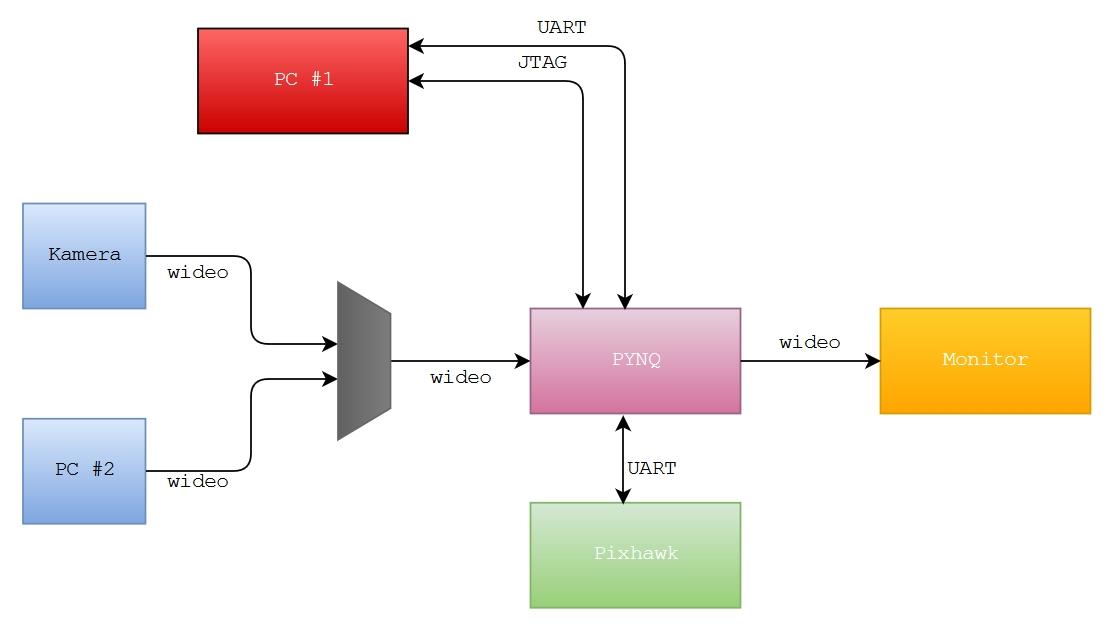
\includegraphics[width=16cm]{6_testing_setup.jpg}
	\caption{Schemat stanowiska testowego}
	\label{fig:testing_setup}
\end{figure}

Na przykładowym materiale wideo zaprezentowano skanowanie obrazu. Niebieskimi prostokątami oznaczone są aktualne okna detekcji dla poszczególnych skal. Zielone okno to obszar śledzenia algorytmem MeanShift, natomiast różowym kolorem oznaczono aktualnie najlepsze okno $128 \times 64$ (przeskalowane ponownie do oryginalnej rozdzielczości).

\begin{figure}[h]
	\centering
	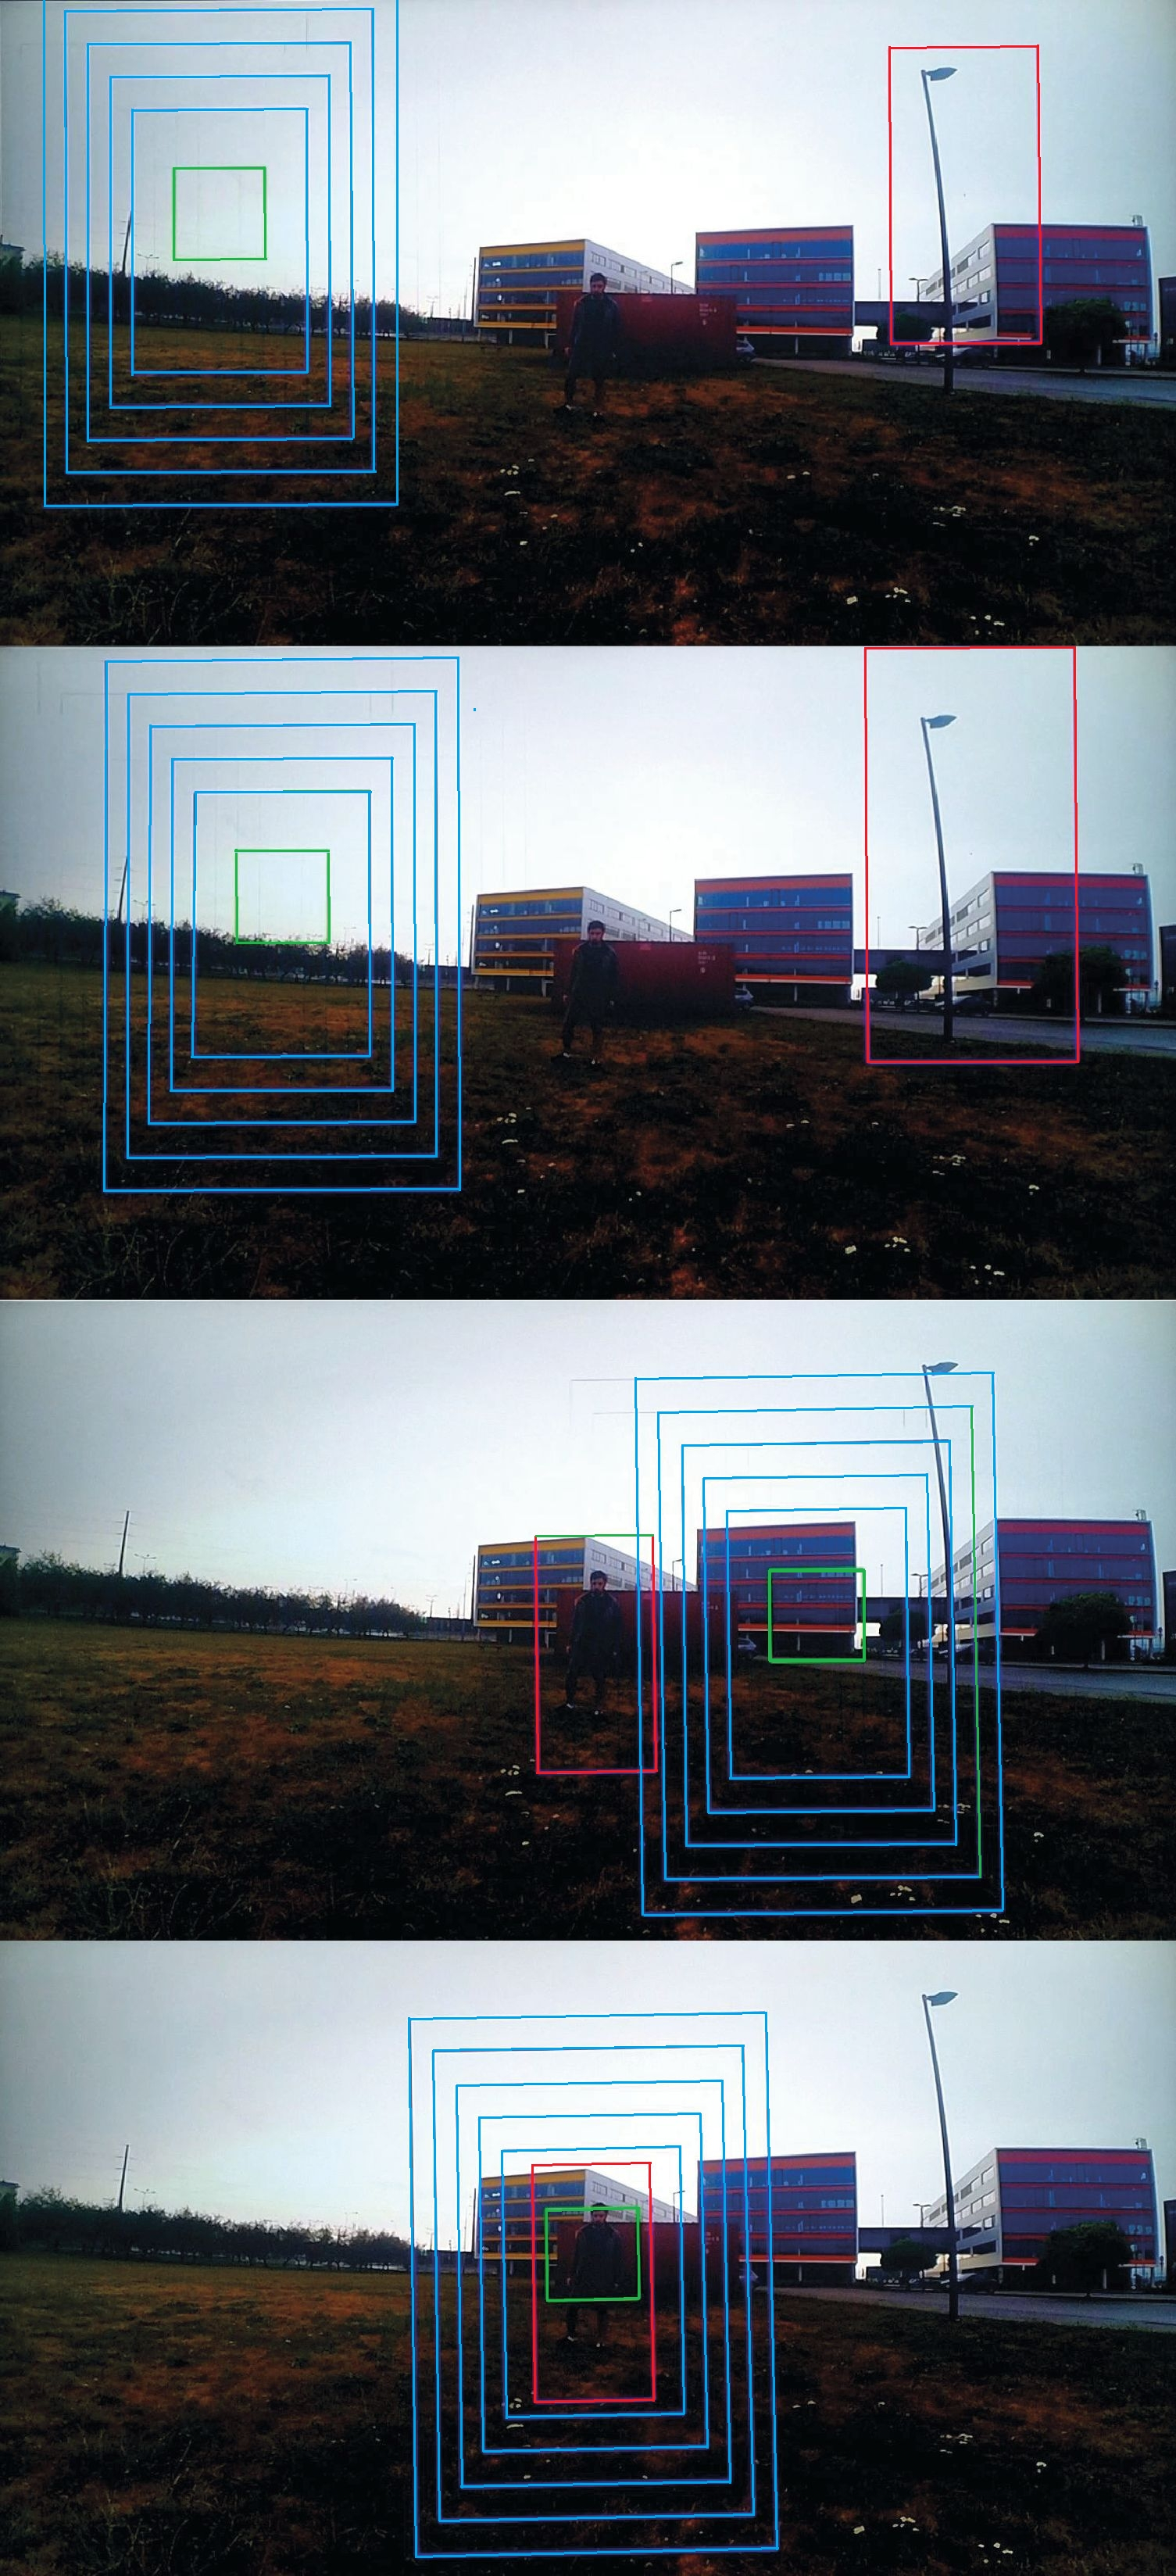
\includegraphics[width=10cm]{6_scan_1.jpg}
	\caption{Proces skanowania}
	\label{fig:scan_screenshot}
\end{figure}

\begin{figure}[h]
	\centering
	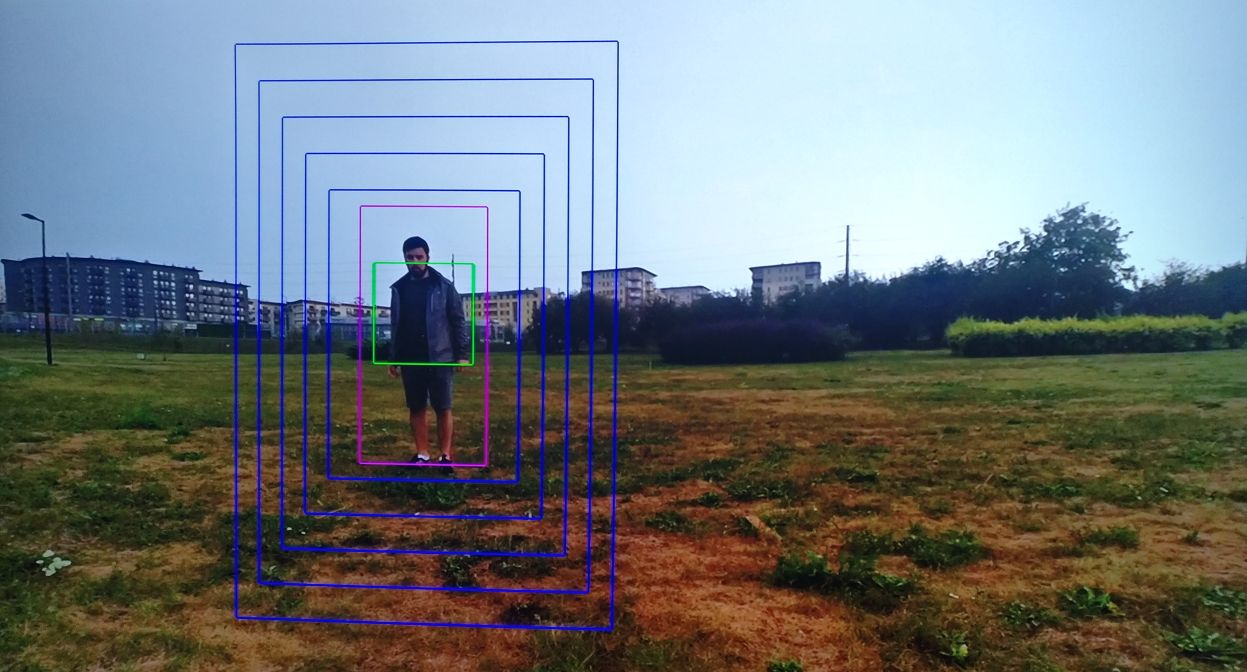
\includegraphics[width=10cm]{6_track_1.jpg}
	\caption{Śledzenie \#1}
	\label{fig:track_1}
\end{figure}

\begin{figure}[h]
	\centering
	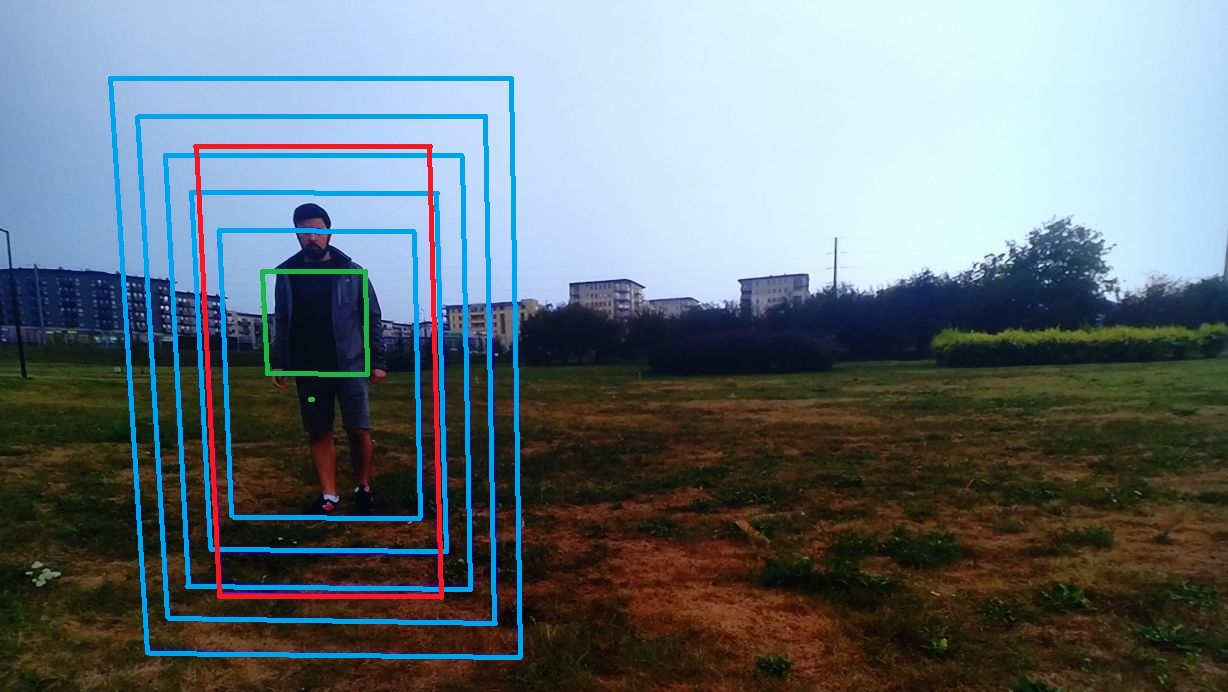
\includegraphics[width=10cm]{6_track_2.jpg}
	\caption{Śledzenie \#2}
	\label{fig:track_1}
\end{figure}

\begin{figure}[h]
	\centering
	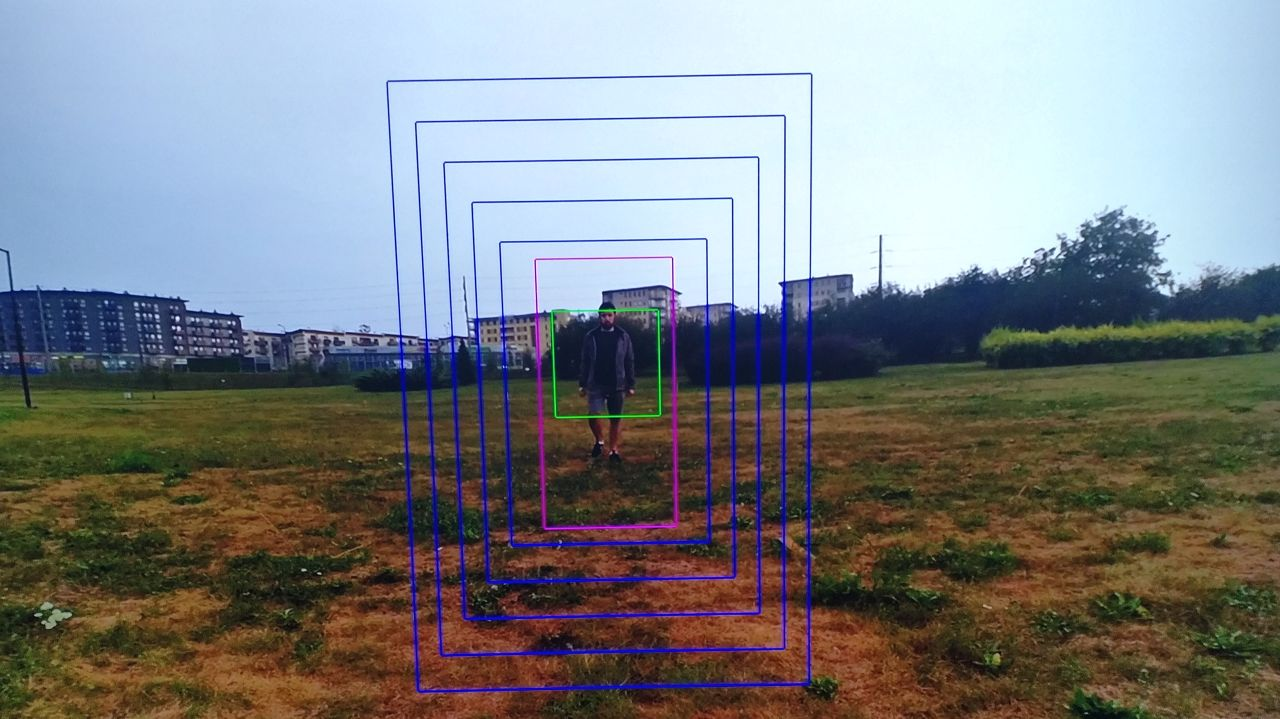
\includegraphics[width=10cm]{6_track_3.jpg}
	\caption{Śledzenie \#3}
	\label{fig:track_1}
\end{figure}

Szczególnie pomocne było wykorzystanie połączenia szeregowego z komputerem, by móc wyświetlić dodatkowe informacje przychodzące z autopilota. Większą część takiego raportu stanowi informacja z PL o odległości od wartości zadanej i skali - przemnożonej przez 10.


\begin{table}[h]
	\centering\scriptsize 
	
	\begin{tabular}{|p{8cm} |}
		
        \hline
prompt>>ARMING... \\
ARMED! \\
TAKING OFF... \\
Sent TAKEOFF CMD. \\
COMMAND ACK: 22 4 \\
STARTING SEARCH! \\
xDiff: 37        \tab yDiff: 33      \tab| scale: 27 || \\
DATA OK, STARTING FOLLOW! \\
xDiff: 20        \tab yDiff: 20      \tab| scale: 25 || \\
xDiff: 10        \tab yDiff: 20      \tab| scale: 25 || \\
xDiff: 52        \tab yDiff: 38      \tab| scale: 22 || \\
xDiff: 94        \tab yDiff: 8       \tab\tab| scale: 22 || \\
xDiff: 140       \tab yDiff: 12      \tab| scale: 20 || \\
xDiff: 165       \tab yDiff: 30      \tab| scale: 25 || \\
xDiff: 157       \tab yDiff: 22      \tab| scale: 22 || \\
xDiff: 125       \tab yDiff: 40      \tab| scale: 25 || \\
xDiff: 95        \tab yDiff: 35      \tab| scale: 22 || \\
xDiff: 62        \tab yDiff: 26      \tab| scale: 20 || \\
xDiff: 26        \tab yDiff: 28      \tab| scale: 20 || \\
xDiff: 10        \tab yDiff: 28      \tab| scale: 20 || \\
xDiff: -6         \tab\tab yDiff: 28      \tab| scale: 20 || \\
xDiff: -30        \tab yDiff: 36      \tab| scale: 20 || \\
xDiff: -70        \tab yDiff: 28      \tab| scale: 20 || \\
xDiff: -86        \tab yDiff: 20      \tab| scale: 20 || \\
xDiff: -118       \tab yDiff: 28      \tab| scale: 20 || \\
xDiff: -150       \tab yDiff: 12      \tab| scale: 20 || \\
xDiff: -150       \tab yDiff: 12      \tab| scale: 20 || \\
xDiff: -110       \tab yDiff: 20      \tab| scale: 20 || \\
xDiff: -86        \tab yDiff: 20      \tab| scale: 20 || \\
xDiff: -62        \tab yDiff: 28      \tab| scale: 20 || \\
INFO: PreArm: Throttle below Failsafe \\
xDiff: 22        \tab yDiff: 28      \tab| scale: 20 || \\
xDiff: 30        \tab yDiff: 4       \tab\tab| scale: 22 || \\
xDiff: 62        \tab yDiff: 42      \tab| scale: 27 || \\
xDiff: 95        \tab yDiff: 33      \tab| scale: 27 || \\
xDiff: 107       \tab yDiff: 33      \tab| scale: 30 || \\
xDiff: 107       \tab yDiff: 33      \tab| scale: 30 || \\
xDiff: 107       \tab yDiff: 33      \tab| scale: 30 || \\
xDiff: 172       \tab yDiff: 34      \tab| scale: 20 || \\
PARAM VAL: 0 1083785216 769  1898664 \\
PARAM VAL: 0 1091798652 769  1898664 \\
xDiff: 268       \tab yDiff: 14      \tab| scale: 20 || \\
xDiff: 368       \tab yDiff: 14      \tab| scale: 22 || \\
xDiff: 450       \tab yDiff: 20      \tab| scale: 25 || \\
xDiff: 560       \tab yDiff: 15      \tab| scale: 22 || \\
Sent LAND CMD. \\
COMMAND ACK: 21 0 \\    
\hline 	
	\end{tabular}
	\caption{Przykładowa zawartość terminala ze śledzenia na podstawie gotowego materiału wideo}
	\label{tab:log}
\end{table}